% ..............................................................................
% Homomorphe Chiffren
% ~~~~~~~~~~~~~~~~~~~~~~~~~~~~~~~~~~~~~~~~~~~~~~~~~~~~~~~~~~~~~~~~~~~~~~~~~~~~~~

\newpage
\hypertarget{homciph}{}
\chapter{Homomorphic Ciphers}
\label{Chapter_HomomorphicCiphers}
\index{homomorphic ciphers}\index{encryption!homomorphic}
(Martin Franz, January 2013)

% -----------------------------------------------------------------------------
\section{Introduction}

Homomorphic ciphers are public-key cryptosystems with special properties. They allow performing certain arithmetic operations on encrypted ciphertexts, without knowing the corresponding plaintexts and without having to decrypt the ciphertexts first. These special properties have led to a huge amount of applications for homomorphic ciphers, e.g. in the domain of cloud computing. A very famous and relatively new cryptosystem with homomorphic properties is the Paillier cryptosystem. But also some of the older and well established cryptosystems, such as ElGamal or RSA, have homomorphic properties.


% -----------------------------------------------------------------------------
\section{Origin of the term ``homomorphic''}

We first clarify the meaning and the origin of the term ``homomorphic''. This term in cryptography is derived from its counterpart in mathematics: in mathematics, a homomorphism is a structure-preserving map between two algebraic structures. In the common sense this means, that a homomorphism $f: X \to Y$ maps the structure of $X$ to the structure of $Y$. Using an example, this can be easily illustrated: Let $(X,+)$ and $(Y,*)$ two algebraic groups with group operations $+$ and $*$, respectively. A homomorphism $f: X \to Y$ maps any given $x \in X$ to a value $y \in Y$, in a way that it holds:
%
$$f(x_1 + x_2) = f(x_1) * f(x_2)$$
%
for any two $x_1, x_2$ in $X$. This means, that for any two values $x_1, x_2$ it does not matter whether we first compute their sum (group operation of $X$) and then apply $f$ (this is the left side of the above given equation); or, whether we first apply $f$ to the values $x_1, x_2$, and then compute their product in $Y$, thus apply the group operation of $Y$. Please note that the operations $+$ and $*$ were chosen here only as an example, they always depend on the algebraic group they belong to. Naturally, the same relation holds for homomorphisms between groups with the same group operation.

\begin{example}{:} Let $X = \mathbb{Z}$ be the set of integer values. The set $\mathbb{Z}$ together with the addition operation forms an algebraic group $G_1 = (\mathbb{Z}, +)$. Similarly, the real values $\mathbb{R}$ without the value zero together with the multiplication operation form a group $G_2 = (\mathbb{R}\backslash\{0\}, *)$. The function $f:\mathbb{Z}{\to}\mathbb{R}\backslash\{0\},z {\to}e^z$ is a homomorphism, since for all $z_1,z_2 \in \mathbb{Z}$ it holds: $f(z_1+ z_2) = e^{(z_1+ z_2 )} = f(z_1 )* f(z_2)$. On the contrary, $f:\mathbb{Z} \to \mathbb{R}\backslash\{0\}, z \to z^2$ is an example for a function which is not a homomorphism.
\end{example}

% -----------------------------------------------------------------------------
\section{Decryption function is a homomorphism}

In the remainder of this chapter we will consider public-key cryptosystems with a special property, namely that its decryption function is a homomorphism. A public-key cryptosystem with this property will be called homomorphic.

Let us for now assume, the above described homomorphism $f$ is the decryption function of a known cryptosystem. This means that we can perform certain algebraic operations in the ciphertext space, knowing which effects this will have on their plaintexts. Following the above given example:

$Y$ corresponds to the set of cipher texts, $X$ is the set of plaintexts. For two plaintexts $x_1, x_2$ with corresponding ciphertexts $y_1, y_2$ it holds:
%
$$f(y_1  * y_2) = f(y_1) + f(y_2) = x_1  + x_2$$
%
This equation can be interpreted as follows: If we multiply two ciphertexts $y_1, y_2$ with each other and subsequently decrypt their product, then we will obtain the sum of the originally encrypted values $x_1$ and $x_2$. Everybody can -- without knowledge of the plaintexts, without having to decrypt and even without knowing the private decryption key -- compute a product of the two ciphertexts and knows that upon decryption the owner of the private key will obtain the sum of the two originally encrypted plaintexts.

% -----------------------------------------------------------------------------
\section{Examples of homomorphic ciphers}

\subsection{Paillier cryptosystem}

The most famous cryptosystem with homomorphic properties is the one by Paillier \cite{hc:Paillier}. First we will see how the Paillier key generation process works. After that, we will show that the Paillier cryptosystem indeed has homomorphic properties.

\subsubsection{Key generation}

First, we generate two random prime numbers $p,q$ in a way that their product $n=pq$ forms  a valid RSA modulus. As for common RSA, the value $n$ should have a bit length of at least 1024 bits.

Using the prime values $p$ and $q$, we can compute the value $\lambda = \textit{lcm}(p-1,q-1)$. $\textit{lcm}$ here denotes the least common multiple. The RSA modulus $n$ will now be the public key, while the private key is the value $\lambda$.

\subsubsection{Encryption}

Let $m$ be the message which will be encrypted, where $m$ is taken from the plaintext space $\mathbb{Z}_n$. For each encryption, we first choose a random element $r$ from the plaintext space $\mathbb{Z}_n$. Subsequently, using the public key, we compute the ciphertext $n$ as:
%
$$c = E(m,r) = (n+1)^m  * r^n  \bmod n^2$$
%
\subsubsection{Decryption}

Given the private key $\lambda$ and a ciphertext $c \in \mathbb{Z}_{n^2}^*$, we first compute $S = c^\lambda \bmod n^2$ and subsequently $T = \phi(n)^{(-1)} \bmod n^2$, where $\phi$ denotes the Euler function.

Finally, we compute the plaintext $m = D(c) = (S-1)/n * T \bmod n$.

\subsubsection{Homomorphic property}

We will now show that the Paillier cryptosystem has the homomorphic property as described above. For this, we will use $E$ to denote the encryption and $D$ to denote the decryption function of the Paillier cryptosystem. For simplicity, we set $g:= n+1$.  For any two plaintexts $m_1,m_2$ and random values $r_1, r_2$ we obtain ciphertexts $c_1, c_2$ as
%
$$c_1 = g^{m_1} *  {r_1}^n \bmod n^2 \mbox{ and } c_2 = g^{m_2} * {r_2}^n \bmod n^2,$$
%
respectively. Now it is easy to see that for the product $c_3 = c_1 * c_2$ it holds
%
$$c_3 = (g^{m_1} * {r_1}^n \bmod n^2) * (g^{m_2} * {r_2}^n \bmod n^2) = g^{m_1+m_2} * (r_1*r_2 )^n \bmod n^2 = E(m_1 + m_2, r_1*r_2)$$
%
Thus, the product of two given ciphertexts is in fact a valid ciphertext, namely the encryption of the sum of the originally encrypted messages. Now it is straightforward to see that the decryption function is a homomorphism. Given two plaintexts $m_1, m_2$ it holds
%
$$D( E(m_1,r_1) * E(m_2,r_2)) = D( E(m_1+m_2, r_1 r_2)) = m_1  + m_2 = D(E(m_1,r_1)) + D(E(m_2,r_2))$$

\subsection{Other cryptosystems}

Also older public-key cryptosystems can have homomorphic properties. Both the ElGamal cryptosystem and RSA constitute famous examples. We will show their homomorphic properties by means of some easy examples.

\subsubsection{RSA}

Let $(e,n)$ be the public RSA key ($e$ the public encryption exponent, $n$ the RSA modulus). For any two messages $m_1, m_2$ we obtain encryptions $c_1 = {m_1}^e \bmod n$ and $c_2 = {m_2}^e \bmod n$. Now for the product of these two encryptions it holds: $c_1*c_2={m_1}^e * {m_2}^e \bmod n=(m_1*m_2)^e \bmod n$. Thus, we obtain an encryption of the product of the two messages $m_1$ and $m_2$. As it is straightforward to see, this property holds for any two plaintexts $m_1, m_2$ and similar as for Paillier, the decryption function is a homomorphism. As we have seen here, RSA is an example for a homomorphism, where both groups have the same group operation.

\subsubsection{ElGamal}

Similar to RSA we can also show the homomorphic properties of the ElGamal cryptosystem. Let $(p,g,K)$ the public key while the private key is $k$ (thus, it holds $g^k \bmod p = K$). For any two messages $m_1, m_2$ and random values $r, s$ we obtain encryptions $(R, c_1) = (K^r \bmod p, m_1*g^r \bmod p)$ and $(S,c_2) = (K^s \bmod p, m_2 * g^s \bmod p)$. As for RSA, we verify that their product $(R*S, c_1*c_2)$ is an encryption of $m_1*m_2$. Again it is straightforward to see that the decryption function is a homomorphism.

% -----------------------------------------------------------------------------
\section{Applications}
The homomorphic property of the Paillier cryptosystem can be used to add two encrypted values or to multiply any value under encryption with a known constant (note that the multiplication corresponds to the repeated application of the addition operation). This makes homomorphic ciphers to important and easy to use base primitives in cryptographic applications.

\begin{enumerate}
\item One of these applications is the so called ``Electronic Voting''. Electronic voting allows a large number of voters to submit their ballots in an encrypted form. This is important in situations, where the voters cannot come together to the same location. This happens, for example, if the voters can only communicate over the internet via email. If the voting behavior of the single parties should remain secret, then the use of homomorphic ciphers is a good solution to this problem. The main principle of electronic voting using homomorphic ciphers is as follows.

All voters encrypt their ballots, using homomorphic encryption (see at the left site of the screenshot). The screenshot depicts the next steps (1 to 3):

\begin{itemize}
\item All voters (on the left in the figure \ref{CT2-PaillierVoting}) encrypt the value 1 if they opt positive and the value 0, if opposed to the decision.
\item Using the homomorphic property, one can compute the sum of all encrypted ballots. Since this happens on encrypted values, the voting behavior of all participants remains secret.
\item At the end, the result of the election is determined and published, this happens by decrypting the sum which was computed using the homomorphic property.
\end{itemize}

\begin{figure}[ht]
\begin{center}
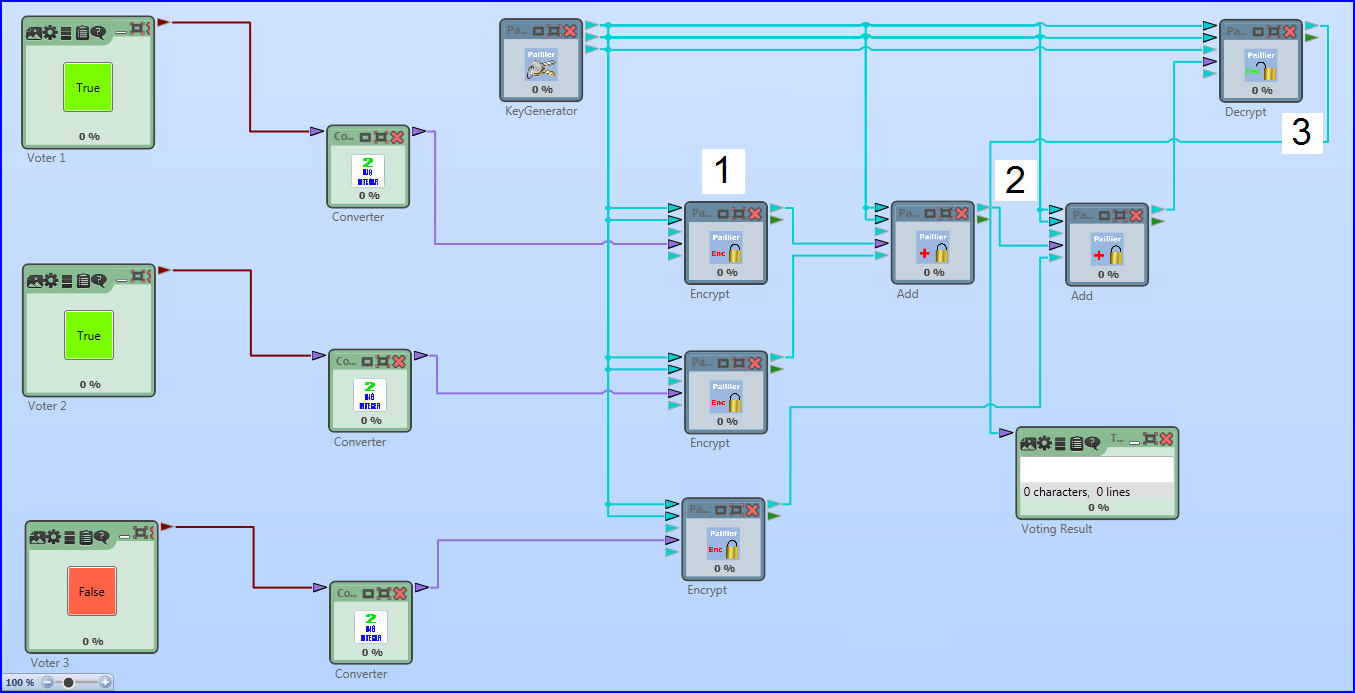
\includegraphics[scale=0.4]{figures/CT2-PaillierVoting.png}
\caption{Voting example for Paillier} 
\label{CT2-PaillierVoting}
\end{center}
\end{figure}

\item A second application of homomorphic ciphers is ``Secure Multiparty Computation''. Here, two or more parties can compute any commonly known function. Each of the parties provides one or more of the inputs for the function to be computed. The goal of the secure computations is to keep all private inputs secret, while only the result of the function is revealed. The use of homomorphic encryption helps to perform these computations on encrypted data. However, since the Paillier encryption only allows to compute additions of encrypted values (and, e.g. no multiplications can be performed), a number of additional methods and techniques have to be applied. The Wikipedia page \cite{hc:SMC} offers a great start for reading more about this topic and more advanced techniques for Secure Multiparty Computation.

\item Furthermore it is expected, that homomorphic encryption will provide great advantages in the areas of ``Cloud Computing''. Using so called ``fully-homomorphic encryption'' \cite{hc:HomEnc} it will be possible to run large applications on external servers only on encrypted data. For this, necessarily one needs to be able to perform both arithmetic operations, the addition and the multiplication, on encrypted data (in contrast to Paillier encryption, which only allows performing additions). Such a crypto system was first presented in 2009 \cite{hc:Gentry2009}.
\end{enumerate}

% -----------------------------------------------------------------------------
\section{Homomorphic ciphers in CrypTool}

\subsection{CrypTool 2}

In CrypTool 2 you will find an implementation of the Paillier cryptosystem. Among the available components, there are components for key generation (Paillier Key Generator), an example for encryption and decryption with Paillier (called Paillier Text), as well as examples which illustrate the homomorphic properties of the cryptosystem (Paillier Addition, Paillier Blinding and Paillier Voting).

\begin{figure}[ht]
\begin{center}
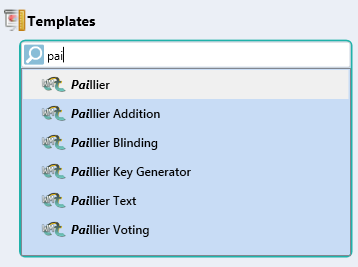
\includegraphics[scale=0.8]{figures/CT2-Paillier.png}
\caption{Paillier cryptosystem in CrypTool 2} 
\label{CT2-Paillier}
\end{center}
\end{figure}

\newpage
\subsection{JCrypTool}

In JCrypTool there is an implementation (see Figure \ref{JCT-HomEnc}), which visualizes the homomorphic properties of various cryptosystem. For RSA and Paillier it shows, that multiplications, for RSA, and additions for Paillier, respectively, can be performed on encrypted values. For the fully-homomorphic cryptosystem by Gentry it is possible to perform both multiplications, as well as additions on encrypted values.

\begin{figure}[ht]
\begin{center}
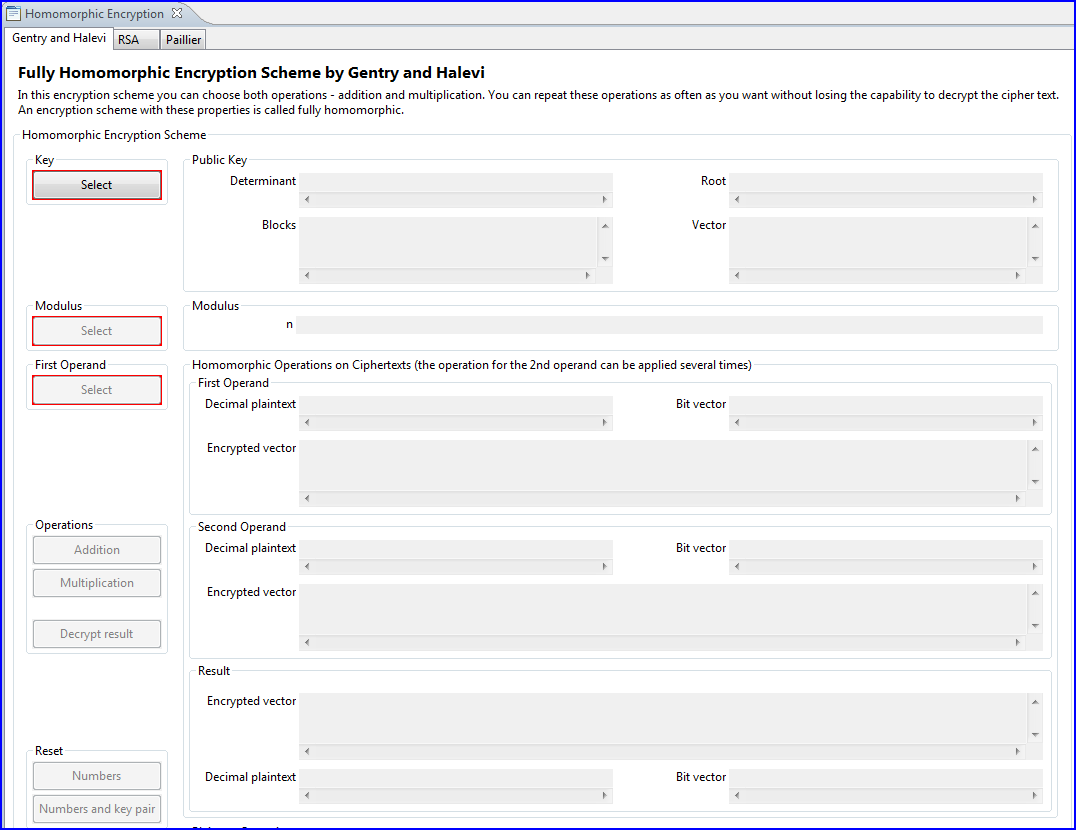
\includegraphics[scale=0.4]{figures/JCT-HomEnc.PNG}
\caption{Visualization of homomorphic properties in JCrypTool} 
\label{JCT-HomEnc}
\end{center}
\end{figure}


%------------------------------------------------------------------------------
\newpage
\begin{thebibliography}{99999}
\addcontentsline{toc}{section}{Bibliography}

\bibitem[Paillier1999]{hc:Paillier} \index{Paillier 1999}
   Pascal Paillier, \\
   {\em Public-Key Cryptosystems Based on Composite Degree Residuosity Classes},\\
	 Advances in Cryptology -- EUROCRYPT'99, 1999.

\bibitem[SMC]{hc:SMC} \index{SMC}
   Wikipedia, \\
   {\em Secure Multiparty Computation}.\\
   \url{http://en.wikipedia.org/wiki/Secure_multi-party_computation}

\bibitem[HomEnc]{hc:HomEnc}
   Wikipedia, \\
   {\em Homomorphic Encryption}\\
   \url{https://en.wikipedia.org/wiki/Homomorphic_encryption}\\
   {\em Homomorphism}\\
   \url{https://en.wikipedia.org/wiki/Homomorphism}

\bibitem[Gentry2009]{hc:Gentry2009} \index{Gentry 2009}
   Craig Gentry, \\
   {\em Fully Homomorphic Encryption Using Ideal Lattices},\\
	In the 41st ACM Symposium on Theory of Computing (STOC), 2009.

\end{thebibliography}  % German

% Local Variables:
% TeX-master: "../script-de.tex"
% End:


